\documentclass[12pt,presentation]{beamer}
\usepackage[utf8]{inputenc}
\usepackage[T1]{fontenc}
\usepackage{fixltx2e}
\usepackage{graphicx}
\usepackage{longtable}
\usepackage{float}
\usepackage{wrapfig}
\usepackage{soul}
\usepackage{textcomp}
\usepackage{marvosym}
\usepackage{wasysym}
\usepackage{latexsym}
\usepackage{amssymb}
\usepackage{hyperref}
\tolerance=1000
\usepackage[english]{babel} \usepackage{ae,aecompl}
\usepackage{mathpazo,courier,euler} \usepackage[scaled=.95]{helvet}
\usepackage{listings}
\lstset{language=Python, basicstyle=\ttfamily\bfseries,
commentstyle=\color{red}\itshape, stringstyle=\color{green},
showstringspaces=false, keywordstyle=\color{blue}\bfseries}
\providecommand{\alert}[1]{\textbf{#1}}

\title{Advanced Python}
\author{FOSSEE}

\usetheme{Warsaw}\usecolortheme{default}\useoutertheme{infolines}\setbeamercovered{transparent}

\AtBeginSection[]
{
  \begin{frame}<beamer>
    \frametitle{Outline}
    \tableofcontents[currentsection]
  \end{frame}
}

\begin{document}

\maketitle

\begin{frame}
\frametitle{Outline}
\setcounter{tocdepth}{3}
\tableofcontents
\end{frame}

\section{Interactive Plotting}

\begin{frame}[fragile]
  \frametitle{First Plot}
  \begin{itemize}
  \item Start IPython with \texttt{-pylab}
  \end{itemize}
  \begin{lstlisting}
    $ ipython -pylab
  \end{lstlisting}  % $
  \begin{lstlisting}
    p = linspace(-pi,pi,100) 
    plot(p, cos(p))
  \end{lstlisting}
\end{frame}


\begin{frame}[fragile]
  \frametitle{\texttt{linspace}}
  \begin{itemize}
  \item \texttt{p} has a hundred points in the range -pi to pi
    \begin{lstlisting}
      print p[0], p[-1], len(p)
    \end{lstlisting}
  \item Look at the doc-string of \texttt{linspace} for more details
    \begin{lstlisting}
      linspace?
    \end{lstlisting}
  \end{itemize}
  \begin{itemize}
  \item \texttt{plot} simply plots the two arguments with default
    properties 
  \end{itemize}
\end{frame}

\section{Embellishing Plots}

\begin{frame}[fragile]
  \frametitle{Plot color and thickness}
  \begin{lstlisting}
    clf()
    plot(p, sin(p), 'r')
  \end{lstlisting}
  \begin{itemize}
  \item Gives a sine curve in Red. 
  \end{itemize}
  \begin{lstlisting}
    plot(p, cos(p), linewidth=2)
  \end{lstlisting}
  \begin{itemize}
  \item Sets line thickness to 2
  \end{itemize}
  \begin{lstlisting}
    clf()
    plot(p, sin(p), '.')
  \end{lstlisting}
  \begin{itemize}
  \item Produces a plot with only points
  \end{itemize}
  \begin{lstlisting}
    plot?
  \end{lstlisting}
\end{frame}

\begin{frame}[fragile]
  \frametitle{\texttt{title}}
  \begin{lstlisting}
    x = linspace(-2, 4, 50)
    plot(x, -x*x + 4*x - 5, 'r', linewidth=2)
    title("Parabolic function -x^2+4x-5")
  \end{lstlisting}
  \begin{itemize}
  \item We can set title using \LaTeX~ 
  \end{itemize}
  \begin{lstlisting}
    title("Parabolic function $-x^2+4x-5$")
  \end{lstlisting} 
\end{frame}

\begin{frame}[fragile]
  \frametitle{Axes labels}
  \begin{lstlisting}
    xlabel("x")
    ylabel("f(x)")
  \end{lstlisting}
  \begin{itemize}
  \item We could, if required use \LaTeX~ 
  \end{itemize}
\end{frame}

\begin{frame}[fragile]
  \frametitle{Annotate}
  \begin{lstlisting}
    annotate("local maxima", xy=(2, -1))
  \end{lstlisting}
  \begin{itemize}
  \item First argument is the annotation text
  \item The argument to \texttt{xy} is a tuple that gives the location
    of the text. 
  \end{itemize}
\end{frame}

\begin{frame}[fragile]
  \frametitle{Limits of Plot area}
  \begin{lstlisting}
    xlim()
    ylim()
  \end{lstlisting}
  \begin{itemize}
  \item With no arguments, \texttt{xlim} \& \texttt{ylim} get the
    current limits
  \item New limits are set, when arguments are passed to them
  \end{itemize}
  \begin{lstlisting}
    xlim(-4, 5)
  \end{lstlisting}
  \begin{lstlisting}
    ylim(-15, 2)
  \end{lstlisting}
\end{frame}

\section{Saving to Scripts}

\begin{frame}[fragile]
  \frametitle{Command history}
  \begin{itemize}
  \item To see the history of commands, we typed
    \begin{lstlisting}
      %hist
    \end{lstlisting}
  \item All commands, valid or invalid, appear in the history
  \item \texttt{\%hist} is a magic command, available only in IPython
  \end{itemize}
  \begin{lstlisting}
    %hist 5
    # last 5 commands
  \end{lstlisting}
  \begin{lstlisting}
    %hist 5-10
    # commands between 5 and 10
  \end{lstlisting}
\end{frame}

\begin{frame}[fragile]
  \frametitle{Saving to a script}
  \begin{itemize}
  \item We wish to save commands for reproducing the parabola
  \item Look at the history and identify the commands that will
    reproduce the parabolic function along with all embellishment
  \item \texttt{\%save} magic command to save the commands to a file
  \end{itemize}
  \begin{lstlisting}
    %save plot_script.py 1 3-6 8
  \end{lstlisting}
  \begin{itemize}
  \item File name must have a \texttt{.py} extension
  \end{itemize}
\end{frame}

\begin{frame}[fragile]
  \frametitle{Running the script}
  \begin{lstlisting}
    %run -i plot_script.py
  \end{lstlisting}
  \begin{itemize}
  \item There were no errors in the plot, but we don't see it!
  \item Running the script means, we are not in interactive mode
  \item We need to explicitly ask for the image to be shown
  \end{itemize}
  \begin{lstlisting}
    show()
  \end{lstlisting}
  \begin{itemize}
  \item \texttt{-i} asks the interpreter to check for names,
    unavailable in the script, in the interpreter
  \item \texttt{sin}, \texttt{plot}, etc. are taken from the
    interpreter
  \end{itemize}
\end{frame}

\section{Saving Plots}

\begin{frame}[fragile]
  \frametitle{\texttt{savefig}}
  \begin{lstlisting}
    x = linspace(-3*pi,3*pi,100)
    plot(x,sin(x))
    savefig('sine.png')
  \end{lstlisting}
  \begin{itemize}
  \item \texttt{savefig} takes one argument
  \item The file-type is decided based on the extension
  \item \texttt{savefig} can save as png, pdf, ps, eps, svg
  \end{itemize}
\end{frame}

\section{Multiple Plots}

\begin{frame}[fragile]
  \frametitle{Overlaid plots}
  \begin{lstlisting}
    x = linspace(0, 50, 10)
    plot(x, sin(x))
  \end{lstlisting}
  \begin{itemize}
  \item The curve isn't as smooth as we expected
  \item We chose too few points in the interval
  \end{itemize}
  \begin{lstlisting}
    y = linspace(0, 50, 500)
    plot(y, sin(y))
  \end{lstlisting}
  \begin{itemize}
  \item The plots are overlaid
  \item It is the default behaviour of \texttt{pylab}
  \end{itemize}
\end{frame}

\begin{frame}[fragile]
  \frametitle{Legend}
  \begin{lstlisting}
    legend(['sine-10 points', 'sine-500 points'])
  \end{lstlisting}
  \begin{itemize}
  \item Placed in the location, \texttt{pylab} thinks is `best'
  \item \texttt{loc} parameter allows to change the location
  \end{itemize}
  \begin{lstlisting}
    legend(['sine-10 points', 'sine-500 points'], 
            loc='center')
  \end{lstlisting}
\end{frame}

\begin{frame}[fragile]
  \frametitle{Plotting in separate figures}
  \begin{lstlisting}
    clf()
    x = linspace(0, 50, 500)
    figure(1)
    plot(x, sin(x), 'b')
    figure(2)
    plot(x, cos(x), 'g')
  \end{lstlisting}
  \begin{itemize}
  \item \texttt{figure} command allows us to have plots separately
  \item It is also used to switch context between the plots
  \end{itemize}
  \begin{lstlisting}
    savefig('cosine.png')
    figure(1)
    title('sin(y)')
    savefig('sine.png')
    close()
    close()
  \end{lstlisting}
  \begin{itemize}
  \item \texttt{close('all')} closes all the figures
  \end{itemize}
\end{frame}

\begin{frame}[fragile]
  \frametitle{Subplots}
  \begin{lstlisting}
    subplot(2, 1, 1)
  \end{lstlisting}
  \begin{itemize}
  \item number of rows
  \item number of columns
  \item plot number, in serial order, to access or create
  \end{itemize}
  \begin{lstlisting}
    subplot(2, 1, 2)
    x = linspace(0, 50, 500)
    plot(x, cos(x))

    subplot(2, 1, 1)
    y = linspace(0, 5, 100)
    plot(y, y ** 2)
  \end{lstlisting}
\end{frame}

\section{Plotting Data}

\begin{frame}[fragile]
  \frametitle{Loading data}
  \begin{itemize}
  \item \texttt{primes.txt} contains a list of primes listed
    column-wise
  \item We read the data using \texttt{loadtxt} 
  \end{itemize}
  \begin{lstlisting}
    primes = loadtxt('primes.txt')
    print primes
  \end{lstlisting}
  \begin{itemize}
  \item \texttt{primes} is a sequence of floats
  \end{itemize}
\end{frame}

\begin{frame}[fragile]
  \frametitle{Reading two column data}
  \begin{itemize}
  \item \texttt{pendulum.txt} has two columns of data
  \item Length of pendulum in the first column 
  \item Corresponding time period in second column
  \item \texttt{loadtxt} requires both columns to be of same length
  \end{itemize}
  \begin{lstlisting}
    pend = loadtxt('pendulum.txt')
    print pend
  \end{lstlisting}
  \begin{itemize}
  \item \texttt{pend} is not a simple sequence like \texttt{primes}
  \end{itemize}
\end{frame}

\begin{frame}[fragile]
  \frametitle{Unpacking with \texttt{loadtxt}}
  \begin{lstlisting}
    L, T = loadtxt('pendulum.txt', unpack=True)
    print L
    print T
  \end{lstlisting}
  \begin{itemize}
  \item We wish to plot L vs. $T^2$
  \item \texttt{square} function gives us the squares
  \item (We could instead iterate over T and calculate)
  \end{itemize}
  \begin{lstlisting}
    Tsq = square(T)

    plot(L, Tsq, '.')
  \end{lstlisting}
\end{frame}

\begin{frame}[fragile]
  \frametitle{\texttt{errorbar}}
  \begin{itemize}
  \item Experimental data always has errors
  \item \texttt{pendulum\_error.txt} contains errors in L and T
  \item Read the values and make an error bar plot
  \end{itemize}
  \begin{lstlisting}
    L, T, L_err, T_err = \
    loadtxt('pendulum_error.txt', unpack=True)
    Tsq = square(T)

    errorbar(L, Tsq , xerr=L_err, 
             yerr=T_err, fmt='b.')
  \end{lstlisting}
\end{frame}

\section{Other kinds of Plots}

\begin{frame}[fragile]
  \frametitle{Scatter Plot}
  \begin{itemize}
  \item The data is displayed as a collection of points
  \item Value of one variable determines position along x-axis
  \item Value of other variable determines position along y-axis
  \item Let's plot the data of profits of a company
  \end{itemize}
  \begin{lstlisting}
    year, profit = loadtxt('company-a-data.txt', 
                            dtype=type(int()))

    scatter(year, profit)
  \end{lstlisting}
  \begin{itemize}
  \item \alert{\texttt{dtype=int}; default is float} 
  \end{itemize}
\end{frame}

\begin{frame}[fragile]
  \frametitle{Pie Chart \& Bar Chart}
  \begin{lstlisting}
    pie(profit, labels=year)
  \end{lstlisting}

  \begin{lstlisting}
    bar(year, profit)
  \end{lstlisting}
\end{frame}

\begin{frame}[fragile]
  \frametitle{Log-log plot}
  \begin{itemize}
  \item Plot a \texttt{log-log} chart of $y=5x^3$ for x from 1 to 20
  \end{itemize}
  \begin{lstlisting}
    x = linspace(1,20,100)
    y = 5*x**3

    loglog(x, y)
    plot(x, y)
  \end{lstlisting}
  \begin{itemize}
  \item Look at \url{http://matplotlib.sourceforge.net/contents.html}
    for more!
  \end{itemize}
\end{frame}


\section{Arrays}

\begin{frame}[fragile]
  \frametitle{Arrays: Introduction}
  \begin{itemize}
  \item Similar to lists, but homogeneous
  \item Much faster than arrays
  \end{itemize}
  \begin{lstlisting}
   In[]: a1 = array([1,2,3,4])
   In[]: a1 # 1-D
   In[]: a2 = array([[1,2,3,4],[5,6,7,8]])
   In[]: a2 # 2-D
  \end{lstlisting}
\end{frame}

\begin{frame}[fragile]
  \frametitle{\texttt{arange} and \texttt{shape}}
  \begin{lstlisting}
   In[]: ar1 = arange(1, 5)
   In[]: ar2 = arange(1, 9) 
   In[]: print ar2
   In[]: ar2.shape = 2, 4
   In[]: print ar2
  \end{lstlisting}
  \begin{itemize}
  \item \texttt{linspace} and \texttt{loadtxt} also returned arrays
  \end{itemize}
  \begin{lstlisting}
   In[]: ar1.shape
   In[]: ar2.shape
  \end{lstlisting}
\end{frame}

\begin{frame}[fragile]
  \frametitle{Special methods}
  \begin{lstlisting}
   In[]: identity(3)
  \end{lstlisting}
  \begin{itemize}
  \item array of shape (3, 3) with diagonals as 1s, rest 0s
  \end{itemize}
  \begin{lstlisting}
   In[]: zeros((4,5))
  \end{lstlisting}
  \begin{itemize}
  \item array of shape (4, 5) with all 0s
  \end{itemize}
  \begin{lstlisting}
   In[]: a = zeros_like([1.5, 1, 2, 3])
   In[]: print a, a.dtype
  \end{lstlisting}
  \begin{itemize}
  \item An array with all 0s, with similar shape and dtype as argument
  \item Homogeneity makes the dtype of a to be float
  \item \texttt{ones, ones\_like, empty, empty\_like}
  \end{itemize}
\end{frame}

\begin{frame}[fragile]
  \frametitle{Operations on arrays}
  \begin{lstlisting}
  In[]:  a1
  In[]:  a1 * 2
  In[]:  a1
  \end{lstlisting}
  \begin{itemize}
  \item The array is not changed; New array is returned
  \end{itemize}
  \begin{lstlisting}
   In[]: a1 + 3
   In[]: a1 - 7
   In[]: a1 / 2.0
  \end{lstlisting}
\end{frame}

\begin{frame}[fragile]
  \frametitle{Operations on arrays \ldots}
  \begin{itemize}
  \item Like lists, we can assign the new array, the old name
  \end{itemize}
  \begin{lstlisting}
   In[]: a1 = a1 + 2
   In[]: a1
  \end{lstlisting}
  \begin{itemize}
   \item \alert{Beware of Augmented assignment!}
  \end{itemize}
  \begin{lstlisting}
   In[]: a, b = arange(1, 5), arange(1, 5)
   In[]: print a, a.dtype, b, b.dtype
   In[]: a = a/2.0
   In[]: b /= 2.0
   In[]: print a, a.dtype, b, b.dtype
  \end{lstlisting}
  \begin{itemize}
  \item Operations on two arrays; element-wise
  \end{itemize}
  \begin{lstlisting}
   In[]: a1 + a1
   In[]: a1 * a2
  \end{lstlisting}
\end{frame}

\section{Accessing pieces of arrays}

\begin{frame}[fragile]
  \frametitle{Accessing \& changing elements}
  \begin{lstlisting}
  In[]:  A = array([12, 23, 34, 45, 56])

  In[]:  C = array([[11, 12, 13, 14, 15],
                    [21, 22, 23, 24, 25],
                    [31, 32, 33, 34, 35],
                    [41, 42, 43, 44, 45],
                    [51, 52, 53, 54, 55]])

   In[]: A[2]
   In[]: C[2, 3]
  \end{lstlisting}
  \begin{itemize}
  \item Indexing starts from 0
  \item Assign new values, to change elements
  \end{itemize}
  \begin{lstlisting}
   In[]: A[2] = -34
   In[]: C[2, 3] = -34
  \end{lstlisting}
\end{frame}

\begin{frame}[fragile]
  \frametitle{Accessing rows}
  \begin{itemize}
  \item Indexing works just like with lists
  \end{itemize}
  \begin{lstlisting}
   In[]: C[2]
   In[]: C[4]
   In[]: C[-1]
  \end{lstlisting}
  \begin{itemize}
  \item Change the last row into all zeros
  \end{itemize}
  \begin{lstlisting}
   In[]:  C[-1] = [0, 0, 0, 0, 0]
  \end{lstlisting}
  OR
  \begin{lstlisting}
   In[]: C[-1] = 0
  \end{lstlisting}
\end{frame}

\begin{frame}[fragile]
  \frametitle{Accessing columns}
  \begin{lstlisting}
  In[]:  C[:, 2]
  In[]:  C[:, 4]
  In[]:  C[:, -1]
  \end{lstlisting}
  \begin{itemize}
  \item The first parameter is replaced by a \texttt{:} to specify we
    require all elements of that dimension
  \end{itemize}
  \begin{lstlisting}
  In[]: C[:, -1] = 0
  \end{lstlisting}
\end{frame}

\begin{frame}[fragile]
  \frametitle{Slicing}
  \begin{lstlisting}
   In[]: I = imread('squares.png')
   In[]: imshow(I)
  \end{lstlisting}
  \begin{itemize}
  \item The image is just an array
  \end{itemize}
  \begin{lstlisting}
   In[]: print I, I.shape
  \end{lstlisting}
  \begin{enumerate}
  \item Get the top left quadrant of the image
  \item Obtain the square in the center of the image
  \end{enumerate}
\end{frame}

\begin{frame}[fragile]
  \frametitle{Slicing \ldots}
  \begin{itemize}
  \item Slicing works just like with lists
  \end{itemize}
  \begin{lstlisting}
  In[]: C[0:3, 2]
  In[]: C[2, 0:3]
  In[]: C[2, :3]
  \end{lstlisting}
  \begin{lstlisting}
  In[]: imshow(I[:150, :150])

  In[]: imshow(I[75:225, 75:225])
  \end{lstlisting}
\end{frame}

\begin{frame}
\frametitle{Image after slicing}
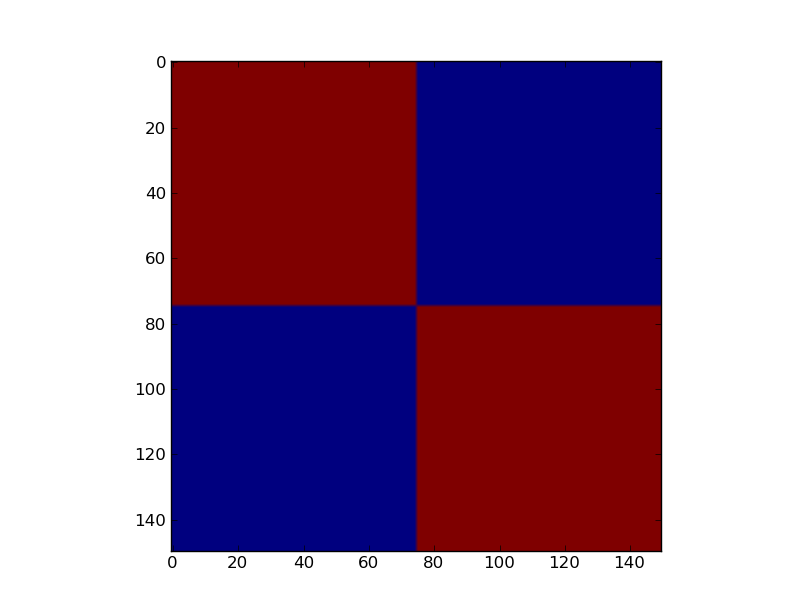
\includegraphics[scale=0.45]{../advanced_python/images/slice.png}\\
\end{frame}



\begin{frame}[fragile]
  \frametitle{Striding}
  \begin{itemize}
  \item Compress the image to a fourth, by dropping alternate rows and
    columns
  \item We shall use striding
  \item The idea is similar to striding in lists
  \end{itemize}
  \begin{lstlisting}
  In[]: C[0:5:2, 0:5:2]
  In[]: C[::2, ::2]
  In[]: C[1::2, ::2]
  \end{lstlisting}
  \begin{itemize}
  \item Now, the image can be shrunk by
  \end{itemize}
  \begin{lstlisting}
  In[]: imshow(I[::2, ::2])
  \end{lstlisting}
\end{frame}

\section{Matrix Operations}

\begin{frame}[fragile]
  \frametitle{Matrix Operations using \texttt{arrays}}
  We can perform various matrix operations on \texttt{arrays}\\ 
  A few are listed below.

  \begin{center}
    \begin{tabular}{lll}
      Operation                    &  How?           &  Example           \\
      \hline
      Transpose                    &  \texttt{.T}       &  \texttt{A.T}         \\
      Product                      &  \texttt{dot}      &  \texttt{dot(A, B)}   \\
      Inverse                      &  \texttt{inv}      &  \texttt{inv(A)}      \\
      Determinant                  &  \texttt{det}      &  \texttt{det(A)}      \\
      Sum of all elements          &  \texttt{sum}      &  \texttt{sum(A)}      \\
      Eigenvalues                  &  \texttt{eigvals}  &  \texttt{eigvals(A)}  \\
      Eigenvalues \& Eigenvectors  &  \texttt{eig}      &  \texttt{eig(A)}      \\
      Norms                        &  \texttt{norm}     &  \texttt{norm(A)}     \\
      SVD                          &  \texttt{svd}      &  \texttt{svd(A)}      \\
    \end{tabular}
  \end{center}
\end{frame}

\section{Least square fit}

\begin{frame}[fragile]
  \frametitle{Least Square Fit}
  \begin{lstlisting}
  In[]:  L, t = loadtxt("pendulum.txt", 
                unpack=True)
  In[]:  L
  In[]:  t
  In[]:  tsq = t * t
  In[]:  plot(L, tsq, 'bo')
  In[]:  plot(L, tsq, 'r')
  \end{lstlisting}
  \begin{itemize}
  \item Both the plots, aren't what we expect -- linear plot
  \item Enter Least square fit!
  \end{itemize}
\end{frame}

\begin{frame}[fragile]
  \frametitle{Matrix Formulation}
  \begin{itemize}
  \item We need to fit a line through points for the equation $T^2 = m \cdot L+c$
  \item In matrix form, the equation can be represented as $T_{sq} = A \cdot p$, where $T_{sq}$ is
    $\begin{bmatrix}
    T^2_1 \\
    T^2_2 \\
    \vdots\\
    T^2_N \\
  \end{bmatrix}$
    , A is   
    $\begin{bmatrix}
    L_1 & 1 \\
    L_2 & 1 \\
    \vdots & \vdots\\
    L_N & 1 \\
  \end{bmatrix}$
    and p is 
    $\begin{bmatrix}
      m\\
      c\\
    \end{bmatrix}$
  \item We need to find $p$ to plot the line
  \end{itemize}
\end{frame}

\begin{frame}[fragile]
  \frametitle{Least Square Fit Line}
  \begin{lstlisting}
  In[]:  A = array((L, ones_like(L)))
  In[]:  A.T
  In[]:  A
  \end{lstlisting}
  \begin{itemize}
  \item We now have \texttt{A} and \texttt{tsq}
  \end{itemize}
  \begin{lstlisting}
  In[]: result = lstsq(A, tsq)
  \end{lstlisting}
  \begin{itemize}
  \item Result has a lot of values along with m and c, that we need
  \end{itemize}
  \begin{lstlisting}
  In[]: m, c = result[0]
  In[]: print m, c
  \end{lstlisting}
\end{frame}

\begin{frame}[fragile]
  \frametitle{Least Square Fit Line}
  \begin{itemize}
  \item Now that we have m and c, we use them to generate line and plot
  \end{itemize}
  \begin{lstlisting}
  In[]:  tsq_fit = m * L + c
  In[]:  plot(L, tsq, 'bo')
  In[]:  plot(L, tsq_fit, 'r')
  \end{lstlisting}
\end{frame}

\begin{frame}
\frametitle{Least Square Fit Line}
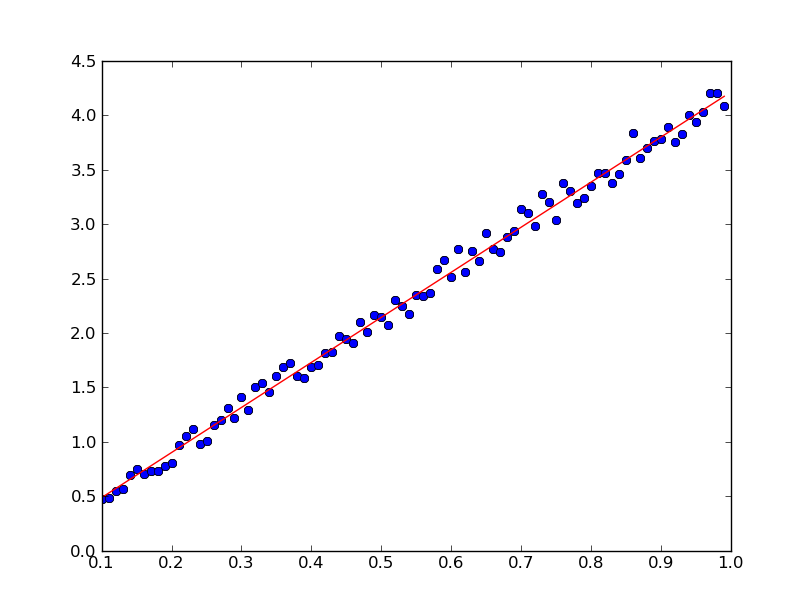
\includegraphics[scale=0.45]{../advanced_python/images/lst-sq-fit.png}\\
\end{frame}



\section{Solving Equations}

\begin{frame}[fragile]
\frametitle{Solution of linear equations}
Consider,
  \begin{align*}
    3x + 2y - z  & = 1 \\
    2x - 2y + 4z  & = -2 \\
    -x + \frac{1}{2}y -z & = 0
  \end{align*}
Solution:
  \begin{align*}
    x & = 1 \\
    y & = -2 \\
    z & = -2
  \end{align*}
\end{frame}

\begin{frame}[fragile]
\frametitle{Solving using Matrices}
Let us now look at how to solve this using \texttt{matrices}
  \begin{lstlisting}
In []: A = array([[3,2,-1],
                  [2,-2,4],                   
                  [-1, 0.5, -1]])
In []: b = array([1, -2, 0])
In []: x = solve(A, b)
  \end{lstlisting}
\end{frame}

\begin{frame}[fragile]
\frametitle{Solution:}
\begin{lstlisting}
In []: x
Out[]: array([ 1., -2., -2.])
\end{lstlisting}
\end{frame}

\begin{frame}[fragile]
\frametitle{Let's check!}
\begin{small}
\begin{lstlisting}
In []: Ax = dot(A, x)
In []: Ax
Out[]: array([  1.00000000e+00,  -2.00000000e+00,  -1.11022302e-16])
\end{lstlisting}
\end{small}
\begin{block}{}
The last term in the matrix is actually \alert{0}!\\
We can use \texttt{allclose()} to check.
\end{block}
\begin{lstlisting}
In []: allclose(Ax, b)
Out[]: True
\end{lstlisting}
\end{frame}

\begin{frame}[fragile]
\frametitle{\texttt{roots} of polynomials}
\begin{itemize}
\item \texttt{roots} function can find roots of polynomials
\item To calculate the roots of $x^2-5x+6$ 
\end{itemize}
\begin{lstlisting}
  In []: coeffs = [1, -5, 6]
  In []: roots(coeffs)
  Out[]: array([3., 2.])
\end{lstlisting}
\vspace*{-.2in}
\begin{center}
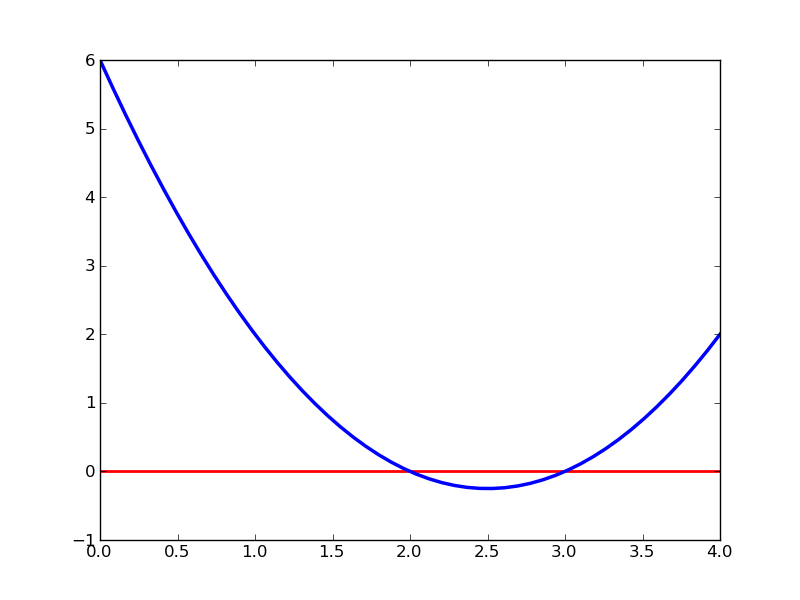
\includegraphics[height=1.6in, interpolate=true]{images/roots}    
\end{center}
\end{frame}

\begin{frame}[fragile]
\frametitle{SciPy: \texttt{fsolve}}
\begin{small}
\begin{lstlisting}
  In []: from scipy.optimize import fsolve
\end{lstlisting}
\end{small}
\begin{itemize}
\item Finds the roots of a system of non-linear equations
\item Input arguments - Function and initial estimate
\item Returns the solution
\end{itemize}
\end{frame}

\begin{frame}[fragile]
\frametitle{\texttt{fsolve} \ldots}
Find the root of $sin(z)+cos^2(z)$ nearest to $0$
\begin{lstlisting}
\begin{lstlisting}
In []: def g(z):
 ....:     return sin(z)+cos(z)*cos(z)

In []: fsolve(g, 0)
Out[]: -0.66623943249251527
\end{lstlisting}
\begin{center}
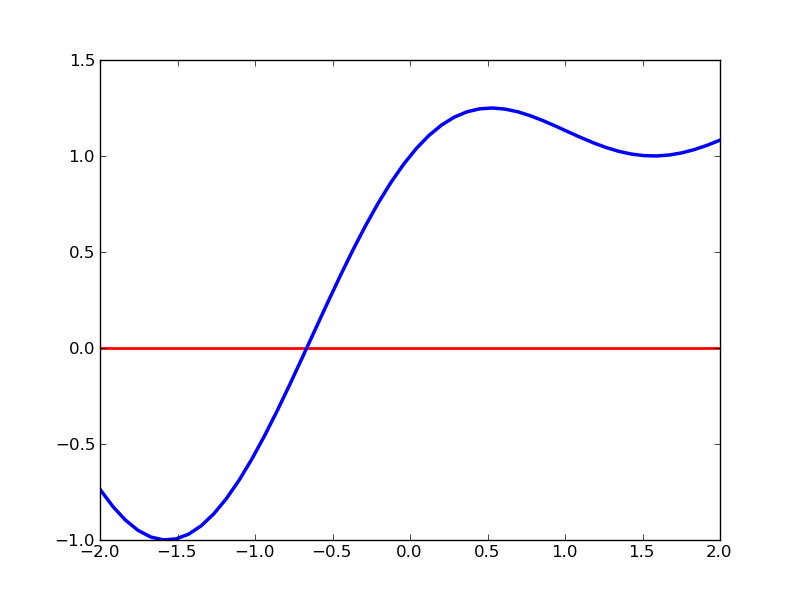
\includegraphics[height=2in, interpolate=true]{images/fsolve}    
\end{center}
\end{frame}

\section{ODEs}

\begin{frame}[fragile]
\frametitle{Solving ODEs using SciPy}
\begin{itemize}
\item Consider the spread of an epidemic in a population
\item $\frac{dy}{dt} = ky(L-y)$ gives the spread of the disease
\item $L$ is the total population.
\item Use $L = 2.5E5, k = 3E-5, y(0) = 250$
\item Define a function as below
\end{itemize}
\begin{lstlisting}
In []: from scipy.integrate import odeint
In []: def epid(y, t):
  ....     k = 3.0e-5
  ....     L = 2.5e5
  ....     return k*y*(L-y)
  ....
\end{lstlisting}
\end{frame}

\begin{frame}[fragile]
\frametitle{Solving ODEs using SciPy \ldots}
\begin{lstlisting}
In []: t = linspace(0, 12, 61)

In []: y = odeint(epid, 250, t)

In []: plot(t, y)
\end{lstlisting}
%Insert Plot
\end{frame}

\begin{frame}[fragile]
\frametitle{Result}
\begin{center}
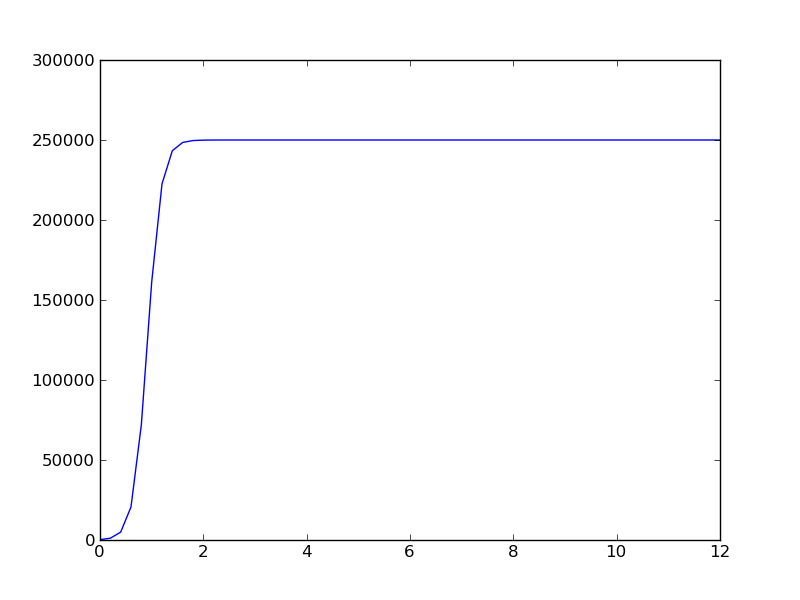
\includegraphics[height=2in, interpolate=true]{images/epid}  
\end{center}
\end{frame}


\begin{frame}[fragile]
\frametitle{ODEs - Simple Pendulum}
We shall use the simple ODE of a simple pendulum. 
\begin{equation*}
\ddot{\theta} = -\frac{g}{L}sin(\theta)
\end{equation*}
\begin{itemize}
\item This equation can be written as a system of two first order ODEs
\end{itemize}
\begin{align}
\dot{\theta} &= \omega \\
\dot{\omega} &= -\frac{g}{L}sin(\theta) \\
 \text{At}\ t &= 0 : \nonumber \\
 \theta = \theta_0(10^o)\quad & \&\quad  \omega = 0\ (Initial\ values)\nonumber 
\end{align}
\end{frame}

\begin{frame}[fragile]
\frametitle{ODEs - Simple Pendulum \ldots}
\begin{itemize}
\item Use \texttt{odeint} to do the integration
\end{itemize}
\begin{lstlisting}
In []: def pend_int(initial, t):
  ....     theta = initial[0]
  ....     omega = initial[1]
  ....     g = 9.81
  ....     L = 0.2
  ....     F=[omega, -(g/L)*sin(theta)]
  ....     return F
  ....
\end{lstlisting}
\end{frame}

\begin{frame}[fragile]
\frametitle{ODEs - Simple Pendulum \ldots}
\begin{itemize}
\item \texttt{t} is the time variable \\ 
\item \texttt{initial} has the initial values
\end{itemize}
\begin{lstlisting}
In []: t = linspace(0, 20, 101)
In []: initial = [10*2*pi/360, 0]
\end{lstlisting} 
\end{frame}

\begin{frame}[fragile]
\frametitle{ODEs - Simple Pendulum \ldots}
%%\begin{small}
\texttt{In []: from scipy.integrate import odeint}
%%\end{small}
\begin{lstlisting}
In []: pend_sol = odeint(pend_int, 
                         initial,t)
\end{lstlisting}
\end{frame}

\begin{frame}[fragile]
\frametitle{Result}
\begin{center}
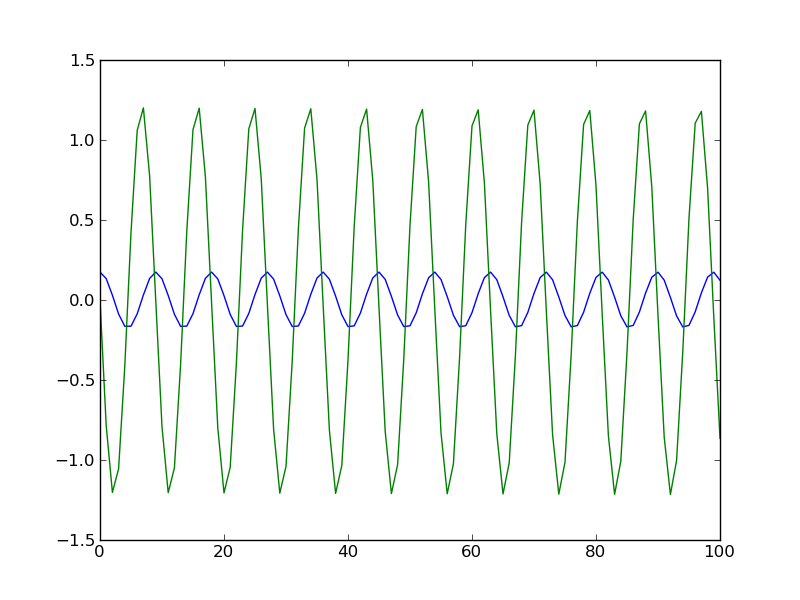
\includegraphics[height=2in, interpolate=true]{images/ode}  
\end{center}
\end{frame}

%% \section{FFTs}

%% \begin{frame}[fragile]
%% \frametitle{The FFT}
%% \begin{itemize}
%%     \item We have a simple signal $y(t)$
%%     \item Find the FFT and plot it
%% \end{itemize}
%% \begin{lstlisting}
%% In []: t = linspace(0, 2*pi, 500)
%% In []: y = sin(4*pi*t)

%% In []: f = fft(y)
%% In []: freq = fftfreq(500, t[1] - t[0])

%% In []: plot(freq[:250], abs(f)[:250])
%% In []: grid()
%% \end{lstlisting} 
%% \end{frame}

%% \begin{frame}[fragile]
%% \frametitle{FFTs cont\dots}
%% \begin{lstlisting}
%% In []: y1 = ifft(f) # inverse FFT
%% In []: allclose(y, y1)
%% Out[]: True
%% \end{lstlisting} 
%% \end{frame}

%% \begin{frame}[fragile]
%% \frametitle{FFTs cont\dots}
%% Let us add some noise to the signal
%% \begin{lstlisting}
%% In []: yr = y + random(size=500)*0.2
%% In []: yn = y + normal(size=500)*0.2

%% In []: plot(t, yr)
%% In []: figure()
%% In []: plot(freq[:250],
%%   ...:      abs(fft(yn))[:250])
%% \end{lstlisting}
%% \begin{itemize}
%%     \item \texttt{random}: produces uniform deviates in $[0, 1)$
%%     \item \texttt{normal}: draws random samples from a Gaussian
%%         distribution
%%     \item Useful to create a random matrix of any shape
%% \end{itemize}
%% \end{frame}

%% \begin{frame}[fragile]
%% \frametitle{FFTs cont\dots}
%% Filter the noisy signal:
%% \begin{lstlisting}
%% In []: from scipy import signal
%% In []: yc = signal.wiener(yn, 5)
%% In []: clf()
%% In []: plot(t, yc)
%% In []: figure()
%% In []: plot(freq[:250], 
%%   ...:      abs(fft(yc))[:250])
%% \end{lstlisting}
%% Only scratched the surface here \dots
%% \end{frame}

\section{Using Python modules}

\begin{frame}[fragile]
  \frametitle{\texttt{hello.py}}
    \begin{itemize}
    \item Script to print `hello world' -- \texttt{hello.py}
    \end{itemize}
    \begin{lstlisting}
    In []: print "Hello world!"
    \end{lstlisting}
    \begin{itemize}
    \item We have been running scripts from IPython
    \end{itemize}
    \begin{lstlisting}
    In []: %run -i hello.py
    \end{lstlisting}
    \begin{itemize}
    \item Now, we run from the shell using python
    \end{itemize}
    \begin{lstlisting}
      $ python hello.py
    \end{lstlisting} %$
\end{frame}

\begin{frame}[fragile]
  \frametitle{Simple plot}
  \begin{itemize}
  \item Save the following in \texttt{sine\_plot.py} 
  \end{itemize}
  \begin{lstlisting}
  In []: x = linspace(-2*pi, 2*pi, 100)
  In []: plot(x, sin(x))
  In []: show()
  \end{lstlisting}
  \begin{itemize}
  \item Now, let us run the script
  \end{itemize}
  \begin{lstlisting}
    $ python sine_plot.py
  \end{lstlisting} % $
  \begin{itemize}
  \item What's wrong?
  \end{itemize}
\end{frame}


\begin{frame}[fragile]
  \frametitle{Importing}
  \begin{itemize}
  \item \texttt{-pylab} is importing a lot of functionality
  \item Add the following to the top of your file
  \end{itemize}
  \begin{lstlisting}
    from scipy import *
  \end{lstlisting}
  \begin{lstlisting}
    $ python sine_plot.py
  \end{lstlisting} % $
  \begin{itemize}
  \item Now, plot is not found
  \item Add the following as the second line of your script
  \end{itemize}
  \begin{lstlisting}
    from pylab import *
  \end{lstlisting}
  \begin{lstlisting}
    $ python sine_plot.py
  \end{lstlisting} % $
  \begin{itemize}
  \item It works!
  \end{itemize}
\end{frame}

\begin{frame}[fragile]
  \frametitle{Importing \ldots}
  \begin{itemize}
  \item \texttt{*} imports everything from \texttt{scipy} and
    \texttt{pylab}
  \item But, It imports lot of unnecessary stuff
  \item And two modules may contain the same name, causing a conflict
  \item There are two ways out
  \end{itemize}
  \begin{lstlisting}
    from scipy import linspace, pi, sin
    from pylab import plot, show
  \end{lstlisting}
  \begin{itemize}
  \item OR change the imports to following and 
  \item Replace \texttt{pi} with \texttt{scipy.pi}, etc. 
  \end{itemize}
  \begin{lstlisting}
    import scipy
    import pylab
  \end{lstlisting}
\end{frame}

\section{Writing modules}

\begin{frame}[fragile]
  \frametitle{GCD script}
  \begin{itemize}
  \item Function that computes gcd of two numbers
  \item Save it as \texttt{gcd\_script.py}
  \end{itemize}
  \begin{lstlisting}
  In []: def gcd(a, b):
    ....    while b:
    ....        a, b = b, a%b
    ....    return a
    ....
  \end{lstlisting}
  \begin{itemize}
  \item Also add the tests to the file
  \end{itemize}
  \begin{lstlisting}
    .... if gcd(40, 12) == 4 and gcd(12, 13) == 1:
       ....  print "Everything OK"
    .... else:
       ....  print "The GCD function is wrong"
  \end{lstlisting}
  \begin{lstlisting}
    $ python gcd_script.py
  \end{lstlisting} % $
\end{frame}

\begin{frame}[fragile]
  \frametitle{Python path}
  \begin{itemize}
  \item In IPython type the following
  \end{itemize}
  \begin{lstlisting}
    import sys
    sys.path
  \end{lstlisting}
  \begin{itemize}
  \item List of locations where python searches for a module
  \item \texttt{import sys} -- searches for file \texttt{sys.py} or
    dir \texttt{sys} in all these locations
  \item So, our own modules can be in any one of the locations
  \item Current working directory is one of the locations
  \end{itemize}
\end{frame}

\begin{frame}[fragile]
  \frametitle{\texttt{\_\_name\_\_}}
  \begin{lstlisting}
    import gcd_script
  \end{lstlisting}
  \begin{itemize}
  \item The import is successful
  \item But the test code, gets run
  \item Add the tests to the following \texttt{if} block
  \end{itemize}
  \begin{lstlisting}
    if __name__ == "__main__":
  \end{lstlisting}
  \begin{itemize}
  \item Now the script runs properly 
  \item As well as the import works; test code not executed
  \item \texttt{\_\_name\_\_} is local to every module and is equal
    to \texttt{\_\_main\_\_} only when the file is run as a script.
  \end{itemize}
\end{frame}



\end{document}
